\documentclass{beamer}
\usetheme{fibeamer}

\makeatletter
\renewcommand\fibeamer@includeLogo[1][]{}
\makeatother

\usepackage[utf8]{inputenc}
\usepackage[main=english, italian]{babel}

\def\mytitle{WiMAX LDPC codes}
\title{\mytitle} %% that will be typeset on the
\subtitle{Complexity and effectiveness} %% title page.
\author{Enrico Lovisotto}

\usepackage{ragged2e}  % `\justifying` text
\usepackage{booktabs}  % Tables
\usepackage{tabularx}
\usepackage{tikz}      % Diagrams
\usetikzlibrary{calc, shapes, backgrounds}
\usepackage{amsmath, amssymb}

\usepackage{mathtools}
\usepackage{url}       % `\url`s
\usepackage{listings}  % Code listings

\usepackage{color}

\frenchspacing
\begin{document}
\setbeamertemplate{caption}{\raggedright\insertcaption\par}
\frame{\maketitle}

\AtBeginSection[]{% Print an outline at the beginning of sections
  \begin{frame}<beamer>
    \frametitle{\mytitle}

    \tableofcontents[currentsection]
  \end{frame}}

\begin{darkframes}
  \section{Specification}
  \subsection{Design}
  \begin{frame}{Design}
    For each code rate, a \textsl{compressed} encoding matrix is specified by the standard: it can then be expanded to suit a specific code length.

    \definecolor{little-grey}{HTML}{515151}
    \def\0{{\color{little-grey} 0}}

    \vspace{-0.5cm}%
    {\renewcommand{\arraystretch}{0.9}
    \begin{equation*}
      \begin{split}
        &\left[ \begin{array}{cc||cc}
          1 & -1 & 1 & -1\\
          2 & 1 & -1 & 1\\
        \end{array} \right] \quad \Longrightarrow \\[0.5em]
      & \Longrightarrow \quad \left[ \begin{array}{c|c||c|c}
          \begin{array}{ccc}
            1 & \0 & \0 \\
            \0 & 1 & \0 \\
            \0 & \0 & 1 \\
          \end{array} &
          \begin{array}{ccc}
            \0 & \0 & \0 \\
            \0 & \0 & \0 \\
            \0 & \0 & \0 \\
          \end{array} &
          \begin{array}{ccc}
            1 & \0 & \0 \\
            \0 & 1 & \0 \\
            \0 & \0 & 1 \\
          \end{array} &
          \begin{array}{ccc}
            \0 & \0 & \0 \\
            \0 & \0 & \0 \\
            \0 & \0 & \0 \\
          \end{array}
          \\ \hline
          \begin{array}{ccc}
            \0 & \0 & 1 \\
            1 & \0 & \0 \\
            \0 & 1 & \0 \\
          \end{array} &
          \begin{array}{ccc}
            1 & \0 & \0 \\
            \0 & 1 & \0 \\
            \0 & \0 & 1 \\
          \end{array} &
          \begin{array}{ccc}
            \0 & \0 & \0 \\
            \0 & \0 & \0 \\
            \0 & \0 & \0 \\
          \end{array} &
          \begin{array}{ccc}
            1 & \0 & \0 \\
            \0 & 1 & \0 \\
            \0 & \0 & 1 \\
          \end{array}
        \end{array} \right]
      \end{split}
    \end{equation*}}
    Each element of \textsl{compressed} version is replaced with a zero matrix if negative and a certain circular right shift of identity matrix otherwise.
    \vspace{0.5cm}
  \end{frame}

  \subsection{Working modes}
  \begin{frame}{Working modes}
    IEEE 802.16e WiMAX specification defines various code lengths and rates.
    All combinations will be further analyzed.

    \vspace{0.5cm}

    \parbox{0.49\linewidth}{
      \begin{table}
        \begin{tabular}{cccc}
          576  & 672  & 768  & 864  \\
          960  & 1056 & 1152 & 1248 \\
          1344 & 1440 & 1536 & 1632 \\
          1728 & 1824 & 1920 & 2016 \\
          2112 & 2208 & 2304 &      \\
        \end{tabular}
        \caption{Code lengths}
      \end{table}
    }
    \parbox{0.49\linewidth}{
      \begin{table}
        \begin{tabular}{ccc} \\ \\ \\
          1/2  & 2/3A & 3/4B \\
          2/3B & 3/4A & 5/6
        \end{tabular}
        \caption{Code rates}
      \end{table}
    }
  \end{frame}

  \section{Simulation}
  \subsection{Encoder}
  \begin{frame}{Encoder}
    \begin{figure}[h]
      \centering
      \includegraphics{figures/encoder.eps}
    \end{figure}
    \begin{equation*}
      c_i = ENC(u_i) =
      \left[
          \begin{array}[h]{c|c}
            u_i & A \, u_i
          \end{array}
        \right]
      \quad \text{where} \quad  \begin{dcases}
        H = \left[
          \begin{array}[h]{c|c}
            B & C
          \end{array}
        \right] \\
       A = C^{-1} B
      \end{dcases}
    \end{equation*}
  \end{frame}

  \subsection{Modulator and channel}
  \begin{frame}{Modulator and channel}
    \begin{figure}[h]
      \centering
      \includegraphics{figures/channel.eps}
      \label{fig:channel_model}
    \end{figure}
    \begin{equation*}
      \begin{split}
        d_i
        = MOD(c_i)
        = & \begin{dcases}
          +1 & c_i = 1 \\
          -1 & c_i = 0
        \end{dcases} \\
        r_i
        = d_i + w_i \quad\text{where}\quad
        & \begin{dcases}
          w_i \sim \mathcal{N}(0, \sigma^2) \\
          \sigma^2 = \left( 2R~ \frac{E_b}{N_o} \right)^{-1}
        \end{dcases}
      \end{split}
    \end{equation*}
  \end{frame}

  \subsection{Decoder}

  \definecolor{my-orange}{HTML}{FFCD64}
  \definecolor{my-green}{HTML}{92FF64}
  \definecolor{my-purple}{HTML}{B164FF}
  \definecolor{my-blue}{HTML}{64C3FF}

  \begin{frame}{Message passing}
    \begin{minipage}{0.7\linewidth}
      \begin{figure}
        \hspace{-0.8cm}%
        
\includegraphics[scale=1.4]{figures/message-passing.eps}
        \caption{FFG of a generic LDPC code}
        \label{fig:phi_tilde}
      \end{figure}
    \end{minipage}%
    \begin{minipage}{0.4\linewidth}
      \begin{equation*}
        \begin{split}
          \textcolor{my-orange}{ch} & ~~ \text{channel information}   \\
          \textcolor{my-blue}{F}    & ~~ \text{forward messages}      \\
          \textcolor{my-purple}{B}  & ~~ \text{backward messages}     \\
          \textcolor{my-green}{b}   & ~~ \text{extrinsic information} \\
        \end{split}
      \end{equation*}
    \end{minipage}
  \end{frame}

  \begin{frame}{Sparse matrix}
    % data structure + performances
    % specific operations implemented
    \begin{figure}[h]
      \centering
      \includegraphics[width=\textwidth]{figures/sparse-matrix.eps}
      \caption{In-memory representation of a generic matrix $A$}
      \label{fig:phi_tilde}
    \end{figure}
  \end{frame}


  \begin{frame}{Function $\tilde{\phi}$}
    \begin{figure}[h]
      \centering
      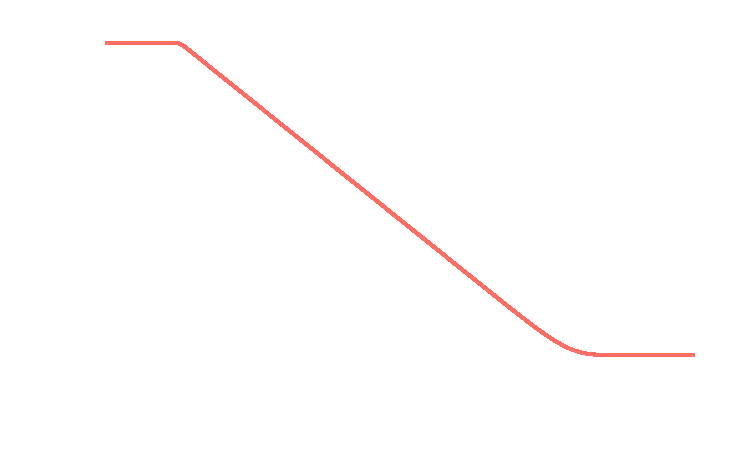
\includegraphics[width=\textwidth]{figures/phi_tilde.pdf}
      \vspace{-1cm}
      \caption{Function is approximated for small and high values of $x$}
      \label{fig:phi_tilde}
    \end{figure}
  \end{frame}

  \section{Results}
  \subsection{Error detection}
  \begin{frame}{Error detection per code length}
    \begin{figure}[h]
      \centering
      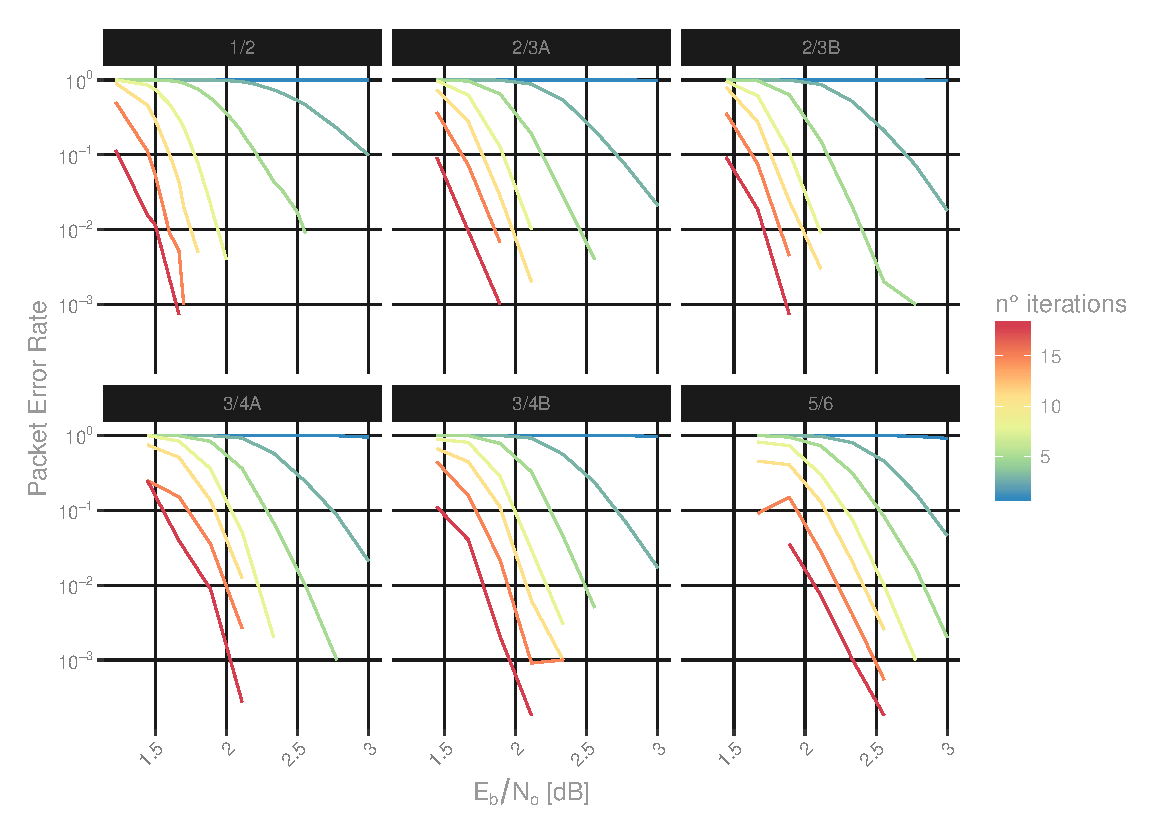
\includegraphics[width=\textwidth]{figures/Pe_vs_SNR_per_length.eps}
    \end{figure}
  \end{frame}

  \begin{frame}{Error detection per code rate}
    \begin{figure}[h]
      \centering
      \vspace{-2mm}%
      \hspace{-6mm}%
      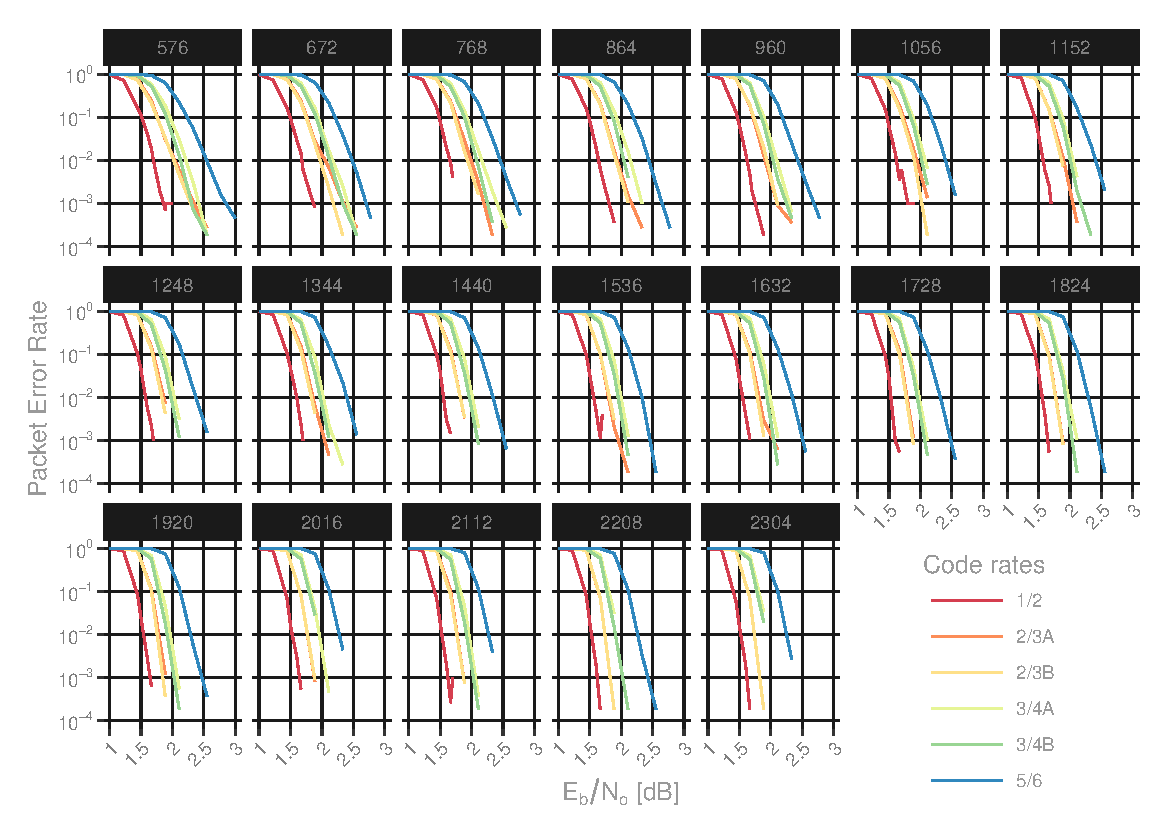
\includegraphics[width=1.05\textwidth]{figures/Pe_vs_SNR_per_rate.eps}
    \end{figure}
  \end{frame}

  \subsection{Sum-product iterations}
  \begin{frame}{Sum-product iterations per code length}
    \begin{figure}[h]
      \centering
      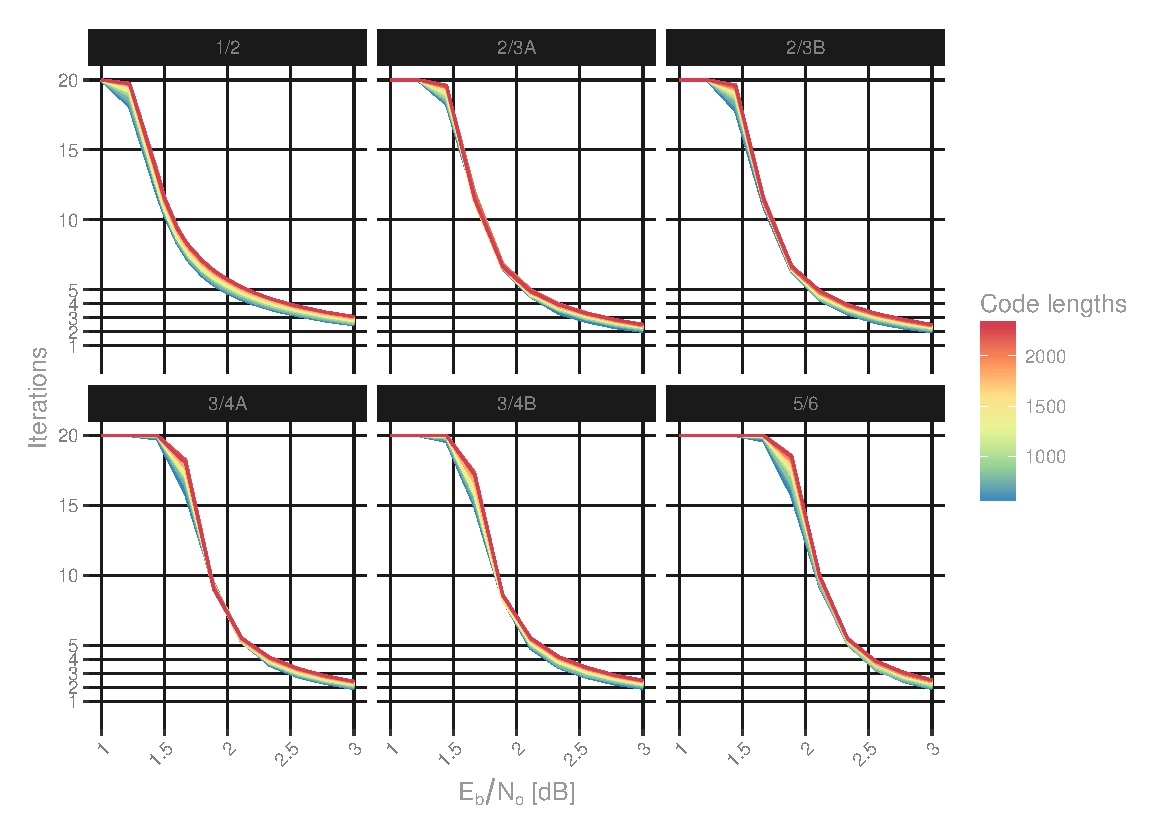
\includegraphics[width=\textwidth]{figures/iters_vs_SNR_per_length.eps}
    \end{figure}
  \end{frame}

  \begin{frame}{Sum-product iterations per code rate}
    \begin{figure}[h]
      \centering
      \vspace{-2mm}%
      \hspace{-6mm}%
      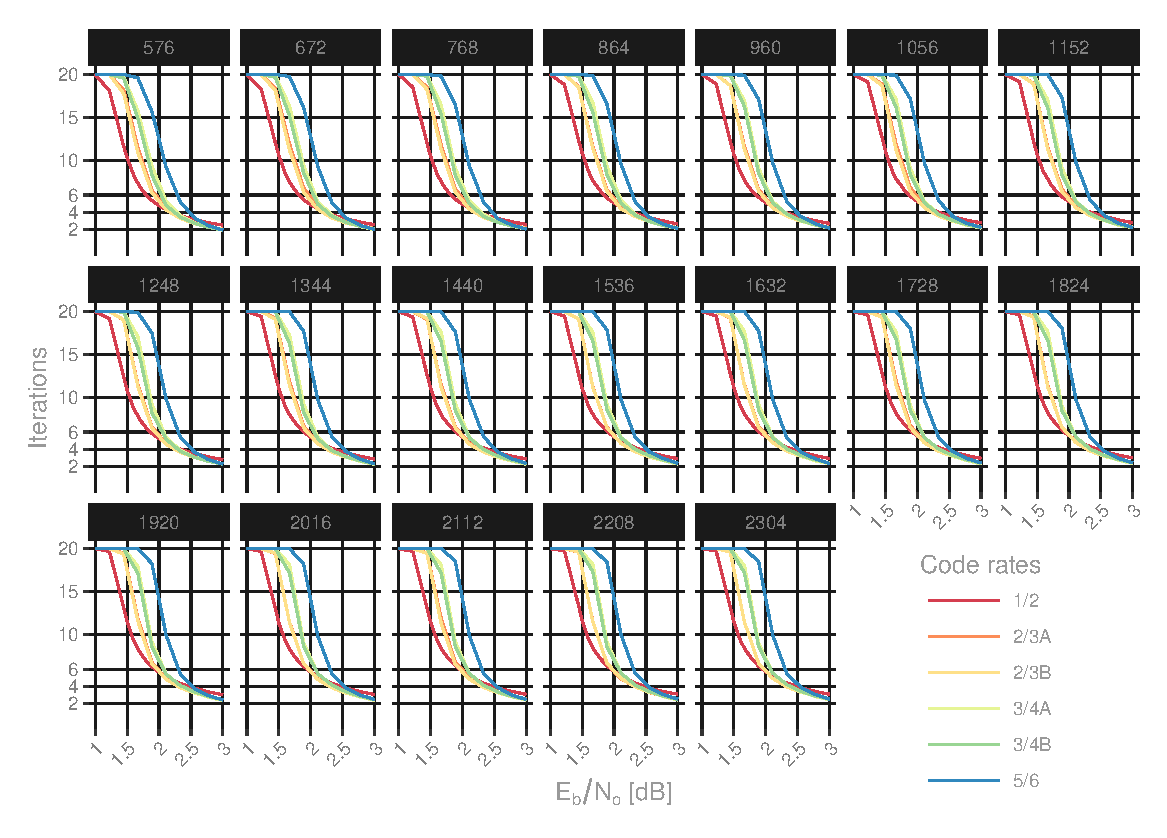
\includegraphics[width=1.05\textwidth]{figures/iters_vs_SNR_per_rate.eps}
    \end{figure}
  \end{frame}

\end{darkframes}

\end{document}

%%% Local Variables:
%%% mode: latex
%%% TeX-master: t
%%% End:
